\graphicspath{{chapters/14/images/}}
\chapter{Quantifying uncertainties and sampling quality}

\section{Introduction}
Dealing with huge system and dealing with a huge amount of data is not sufficient to interpret the biological relevance of a molecular definition.
There is a need to perform thoughtful analysis on the obtained data.
Data interpretation is a fundamental step to asses the validity of a simulation.
The methods presented in this chapter will be useful also when dealing with Monte Carlo simulations, although the simulation is more difficult to interpret as time becomes moves.

	\subsection{Key definitions}

		\subsubsection{Expectation value}
		The Expectation value is defined as:

		$$\langle x\rangle = \int xP(x)dx = \sum\limits_jx_jP(x_j)$$

		In the case of molecular dynamics simulations time will be discretized, so the probability distribution will be discretized.

		\subsubsection{Estimate of expectation value}
		The estimate of the expectation value, or arithmetic mean is computed as:

		$$\bar{x} = \frac{1}{n}\sum\limits_{j=1}^nx_j$$

		\subsubsection{Variance}
		The variance is computed as:

		$$\sigma^2_x = \int dxP(x)(x-\langle x\rangle)^2 = \sum\limits_{j}P(x_j)\bigl(x_j-\langle x\rangle\bigr)^2$$

		\subsubsection{Standard deviation}
		The standard deviation is $\sigma_x$ and its estimate is the experimental standard deviation:

		$$s(x) = \sqrt{\frac{\sum\limits_{j=1}^n(x_j-\bar{x})^2}{n-1}}$$

		The estimates are necessary in molecular dynamics as the probability distribution is not known.

		\subsubsection{Linear correlation}
		Two variables are defined as linearly uncorrelated observables:

		$$\bigl\langle(x-\langle x\rangle)(y-\langle y\rangle)\bigr\rangle = 0$$

		Linear uncorrelation does not imply independent variables.

		\subsubsection{Experimental standard deviation}
		The experimental standard deviation of the mean is computed as:

		$$s(\bar{x}) = \frac{s(x)}{\sqrt{n}}$$

		If all the $x_j$ are assumed to be linearly uncorrelated, this is used to estimate error in computer simulations.

		\subsubsection{Correlation time}
		The correlation time $\tau$ is the longest separation time $\Delta t$ over which $x(t)$ and $x(t + \Delta t)$ remain linearly correlated.
		This is important as only data that are separated more than the correlation time are linearly uncorrelated and can be used when computing the standard deviation of mean.
		If they would be included the standard deviation would be underestimated.

		\subsubsection{Two sided confidence interval}
		Once the standard deviation is computed the two-sided confidence interval can be obtained: $\langle x\rangle = \bar{x} \pm U$ with $U = ks(\bar{x})$ and $k$ the coverage factor for a given level of confidence $p$ expressed in percentage.
		Usually $k=2$ to obtain a level of confidence about $95\%$, so that the expectation value is expected with $95\%$ probability to lie in the interval.
		This is the ideal situation, but there is no certainty that the molecular simulation will explore the entirety of the phase-space compatible with the macroscopic conditions.

	\subsection{Time scales}
	Before starting a simulation the time scale of the process of interest has to be estimated.
	For instance, looking at protein folding, obtained through experimental measure, the time scale could change from microseconds to minutes depending on the dimension of the protein.
	The latter case cannot be explored with a standard molecular simulation, so a coarse-grained model or other methods should be used to accelerate the dynamics (using approximations out of control, biasing the dynamics).

	\begin{figure}[H]
		\centering
		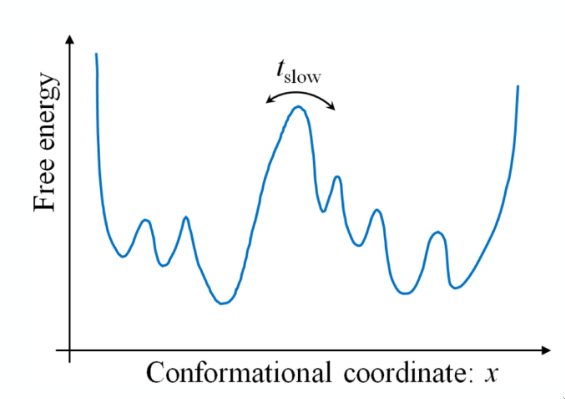
\includegraphics[scale = 0.4]{time-scales}
		\caption{Time scales}
		\label{fig:time-scales}
	\end{figure}

	Figure \ref{fig:time-scales} depicts a free energy profile.
	Usually when starting a simulation the starting point is a minimum.
	Sampling the simulation for a long time a transition to other minima could be observed, but these processes that happen to processes that happen on a faster time-scale with respect to processes that need to surpass a higher energy barrier.
	The time-scale of the transition depends exponentially on the height of the transition, so the higher the barrier the longer the time to observe the transition.
	Whenever a simulation is started an estimate of the slowest time scale involved in the process need to be understood.



\section{Equilibration}
When performing a simulation it is fundamental to consider if the simulation is equilibrated enough, so if the system has equilibrated after the simulation.
This is very difficult to understand, but it is easy to tell if a system is non-equilibrated.
Some of the variables that can be checked to see for non-equilibration are scalar values:

\begin{multicols}{2}
	\begin{itemize}
		\item System size which depends on the ensemble: in the case of NPT it is important.
			If it is equilibrated the volume would fluctuate around an average.
		\item Membrane area for membrane proteins: when simulating a protein at the beginning the membrane adapt to the protein and after a while equilibration is reached and area per lipid does not change and so does total membrane area.
		\item Potential energy or total energy, this is expected to fluctuate around an average value.
			At the beginning it varies due to temperature or initial configuration before reaching an average, so it as equilibrated in a local minimum of an average.
		\item Temperature in the NVE ensemble, so temperature will be constant when the system is at equilibrium.
		\item Density of simulated molecules in the NPT ensemble.
		\item Pressure, not recommended because in pressure there are huge variation because it depends on the Virial, so the average value will be $1 atm$, but the fluctuation will be huge.
		\item Radius of gyration is an overall information on the protein structure.
			There is the possibility to reach the same value in different conformation, a problem that applies to other overall distance measures.
			Even if there are conformation with the same value of gyration they could be different.
			If the radius of gyration is constantly increasing or decreasing the simulation has not equilibrated yet.
		\item Configurational distance measures like RNMS, all-to-all RMSD map.
			The discussion for radius of gyration holds for this measures.
			Considering RMSD:

			$$RMSD(\vec{r}, \vec{s}) = \sqrt{\frac{1}{N}\sum\limits_{i=1}^N|\vec{r}_i-\vec{s}_i|^2}$$

			This will reach a constant value with some fluctuation.
			The all-to-all RMSD map checks the RMSD for all the conformation present in the molecular dynamics simulation, obtaining a matrix of distances that can be plotted as in \ref{all-to-all-rmsd}.
	\end{itemize}
\end{multicols}

\begin{multicols}{2}

	\begin{figure}[H]
		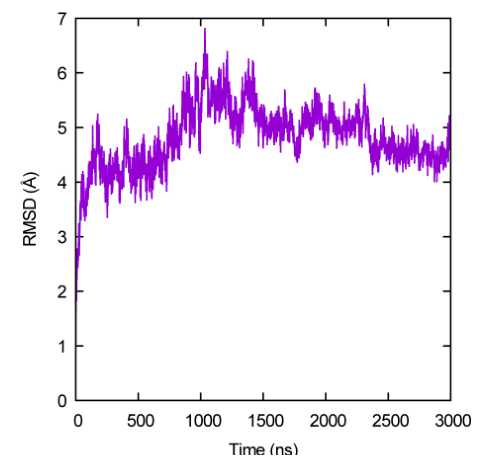
\includegraphics[width = 0.45\textwidth]{rmsd}
		\caption{RMSD}
		\label{fig:rmsd}
	\end{figure}

	\columnbreak

	\begin{figure}[H]
		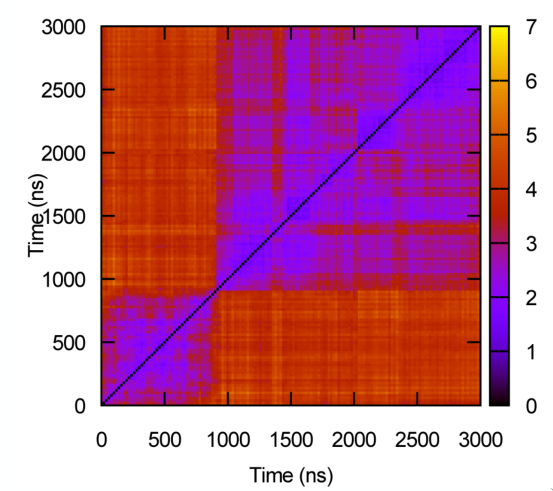
\includegraphics[width = 0.45\textwidth]{all-to-all-rmsd}
		\caption{All-to-all RMSD map, in blue low values and in red high value}
		\label{fig:all-to-all-rmsd}
	\end{figure}

\end{multicols}

It is very difficult to interpret data from \ref{fig:rmsd}, but it is easier in \ref{fig:all-to-all-rmsd}.
Looking at the latter two conformations can be seen, where there are the basins.
It can be seen how once the protein exits from the lower basin it does not come back and goes into the other.
Moreover in the bigger basis different conformation can be seen that are easily traversed.
This two basin are expected with starting with crystal's coordinate the first is the local basin corresponding to the crystal structure, which can be biased.

	\subsection{Qualitative behaviour}

	\begin{figure}[H]
		\centering
		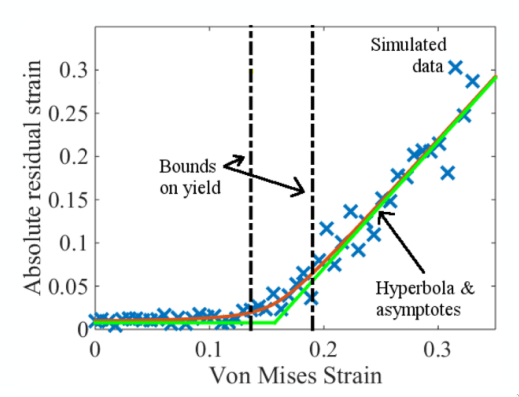
\includegraphics[scale=0.5]{qualitative-behaviour}
		\caption{Qualitative behaviour}
		\label{fig:qualitative-behaviour}
	\end{figure}

	Knowing some qualitative features of the simulation can allow for a more constructive analysis of the data.
	Looking at \ref{fig:qualitative-behaviour} a simulation of a material is considered.
	In this case an expected behaviour is seen and then the simulated data is fitted into a known function, so in this case the expected behaviour is being reproduced, meaning that the simulation has provided good results.

	\subsection{Independent simulations}
	In principle a set of independent simulations should be run.
	Most of the time running independent simulation is not a good choice in the case of protein.
	This is because all the independent simulation are independent only in the velocities: the coordinates are the same not considering the solvent.
	This is very computational expensive, so a more efficient way would be to run long simulation starting from equilibrating structure and randomizing the velocities.

		\subsubsection{Autocorrelation analysis}
		Another method is to start from a single simulation and perform an autocorrelation analysis, to asses whether two snapshots of the simulation are independent.
		To do so the autocorrelation of two quantities like RMSD is computed:

		$$C(x_k, x_{k+j}) \equiv\frac{\bar{(x_k-\bar{x})(x_{k+j}-\bar{x})}}{s^2(x)}\Rightarrow C_j$$

		Where:

		\begin{multicols}{2}
			\begin{itemize}
				\item $x_c$ is data point at time $c$.
				\item $\bar{x}$ is the arithmetic mean.
			\end{itemize}
		\end{multicols}

		This would be done for all the $k$ values and if it does not depend by $k$ but only on $j$ the property has been equilibrated.
		If the function depends on $k$ the simulation has equilibrated.

		\subsubsection{Combined clustering}
		Combined clustering as in \ref{fig:independent_simulation}.
		In combined clustering a measure of the distance of the conformation.
		Then using one clustering algorithm the conformations will be clustered.
		There will be a number of cluster.
		Assume doing so for two independent simulations, or for two part of a long simulation, called in \ref{fig:independent_simulation} $1$ and $2$.
		Then for each of this two simulation the time the simulation spent in one cluster is computed for each cluster.
		This is plotted in the data.
		If the point are off-diagonal the trajectories are not the same so the system has not equilibrated.

		\begin{figure}[H]
			\centering
			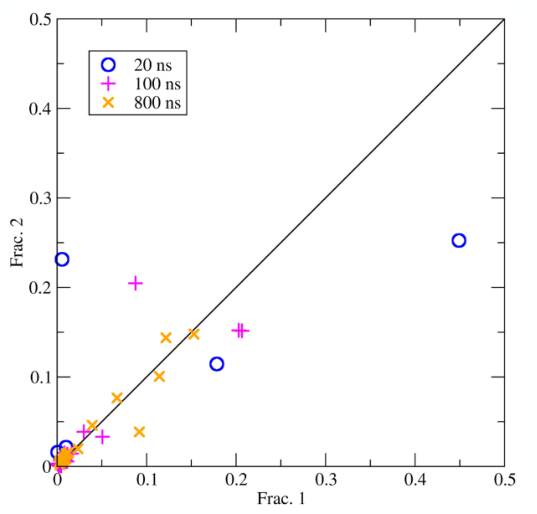
\includegraphics[scale = 0.4]{independent-simulations}
			\caption{Combined clustering}
			\label{fig:independent_simulation}
		\end{figure}

	\subsection{Equilibration and production}
	It can be seen in the case of slowly-equilibrating of figure \ref{fig:equilibration} a drift can be observed so there is no certainty of equilibration.

	\begin{figure}[H]
		\centering
		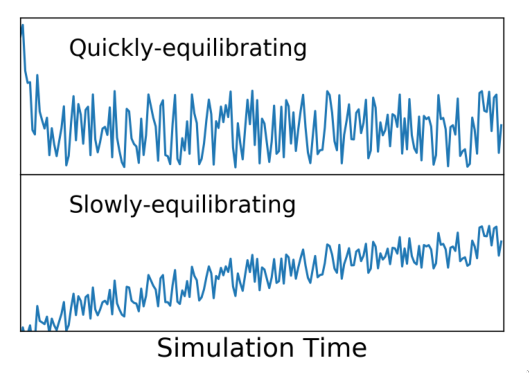
\includegraphics[scale = 0.5]{equilibration}
		\caption{Behaviour during equilibration}
		\label{fig:equilibration}
	\end{figure}

	Once we are confident that equilibration has been reached the trajectory has to be separated into the equilibration and production part.
	This can be seen in \ref{fig:equilibration-production}.
	Now equilibration is discarded and no longer considered in the analysis.
	In the analysis just the production will be considered.

	\begin{figure}[H]
		\centering
		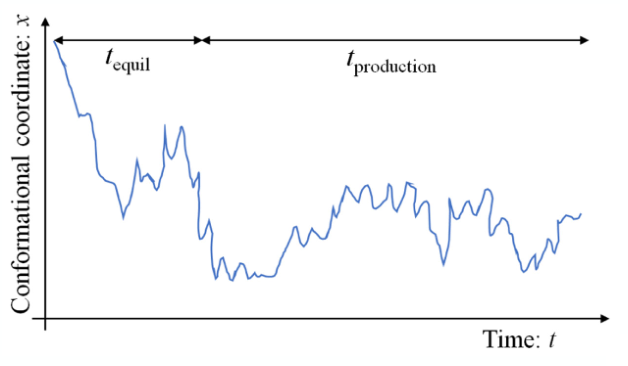
\includegraphics[scale = 0.5]{equilibration-production}
		\caption{Comparison of equilibration and production}
		\label{fig:equilibration-production}
	\end{figure}

	\subsection{Equilibration workflows}
	For the equilibration there are different type of workflow and the choice depends on the system in use.

		\subsubsection{First workflow}
		In this first workflow the simulated times are the physical time as in the NVE ensemble the Hamiltonian dynamics are considered because there is no thermostat.
		So this is a good workflow for observing dynamical properties.

		$$\overbrace{\underbrace{NVT}_{\substack{\text{short simulation to}\\\text{relax to temperature}\\\text{of interest}}}\rightarrow \underbrace{NVE}_{\text{short equilibration}}}^{\text{Suggested equilibration workflow}}\rightarrow \overbrace{NVE}^{\text{Production ensemble}}$$

		\subsubsection{Second workflow}
		In this second workflow the volume is kept fixed, the first simulation is used to adapted to the temperature and then the simulation is run.
		In this case the simulation is run at fixed density.
		This would be used for a liquid material.


		$$\overbrace{\underbrace{NVT}_{\substack{\text{short simulation to}\\\text{relax to temperature}\\\text{of interest}}}}^{\text{Suggested equilibration workflow}}\rightarrow \overbrace{\underbrace{NVT}_{\text{at known, fixed density}}}^{\text{Production ensemble}}$$


		\subsubsection{Third workflow}
		This third workflow is typical for proteins.
		So a combination of NPT and NVT to converge the volume and then the system is simulated without a barostat.

		$$\overbrace{\underbrace{NVT}_{\substack{\text{short simulation to}\\\text{relax to temperature}\\\text{of interest}}}\rightarrow \underbrace{NPT}_{\substack{\text{short simulation to}\\\text{relax to density of}\\\text{interest}}}\rightarrow\underbrace{NPT}_{\substack{\text{to compute average}\\\text{box size}}}\rightarrow \underbrace{NVT}_{\text{short equilibration}}}^{\text{Suggested equilibration workflow}}\rightarrow\overbrace{\underbrace{NVT}_{\substack{\text{for density defined by}\\\text{ pressure or unknown system}\\\text{density distribution,}\\\text{like a homogeneous system}}}}^{\text{Production ensemble}}$$

		\subsubsection{Forth workflow}
		This is a typical simulation for a membrane protein.

		$$\overbrace{\underbrace{NVT}_{\substack{\text{short simulation to}\\\text{relax to temperature}\\\text{of interest}}}\rightarrow \underbrace{NPT}_{\substack{\text{short simulation to}\\\text{relax to density of}\\\text{interest}}}}^{\text{Suggested equilibration workflow}}\rightarrow	\overbrace{NPT}^{\text{Production ensemble}}$$

\section{Autocorrelation}

	\subsection{Autocorrelation function}
	The autocorrelation function is useful to understand whether a system is equilibrated enough and how many independent conformations there are in the analysis.
	This is possible only when the correlation time is computed for an observable.
	So there is an autocorrelation function and time for each observable.
	Let $f(x)$ an observable, a function of the coordinates or the momenta.
	Then the autocorrelation function:

	$$C_f(t') = \frac{\bigl\langle(f(x)-\langle f\rangle)(f(t+t') - \langle f\rangle)\bigr\rangle}{\sigma^2_f}$$

	When $t'=0$ $C_f(t') = 1$.
	This function will decrease with $t'$.
	Using both the equilibration and production part of the simulation $C_f(t')$ will also depend on time time $t$.
	Using only the production run the dependence of $t$ is lost and the autocorrelation function can be computed.
	The function will go to $0$ with an exponential behaviour and fluctuate around that value.
	Performing this on a discretized time and the time ordered sequence of values $f_j = f(t=j\Delta t)$:

	$$C_f(t') = \frac{1}{\sigma^2_f}\frac{1}{N}\sum\limits_{j=1}^{N-\frac{t'}{\Delta t}}(f(j\Delta t)-\langle f\rangle)(f(j\Delta t + t')-\langle f\rangle)$$

	Computing the autocorrelation function starting after an increasing time if the system has equilibrated within the first time chosen the curves superimpose in the first part.

	\subsection{Autocorrelation time}
	The autocorrelation time is defined as:

	$$\tau_f = \int_0^{+\infty} dt' C_f(t')$$

	If the autocorrelation function is an exponential this is a good way to estimate the autocorrelation time.
	Looking at figure \ref{fig:autocorrelation-time}, although it seems that after $200ps$ the autocorrelation time is reached in this way the number of independent conformation is obtained.
	It could be that this number is not sufficient to sample the system properly.
	In that case the system is spending too much time in one conformation and not according to the Boltzmann distribution.
	The autocorrelation time will provide an idea on how many independent conformation there are in the syste,

	\begin{figure}[H]
		\centering
		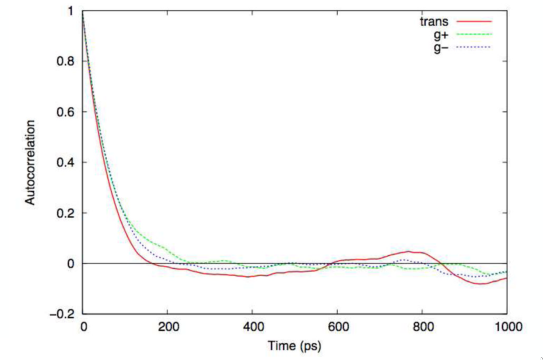
\includegraphics[scale = 0.6]{autocorrelation-time}
		\caption{Autocorrelation time}
		\label{fig:autocorrelation-time}
	\end{figure}

	The autocorrelation time $\tau_f$ is specific for each observable $f$ and allows to obtain the number of independent values of $f$ in the simulation:

	$$N_f^{ind}\simeq\frac{t_{sim}}{\tau_f}$$

	Where $t_{sim}$ is the total simulation time.
	Once the number of independent value is estimated the standard deviation of the mean can be computed using this number:

	$$SE(f) = \frac{\sigma_f}{\sqrt{N_f^{ind}}}\sim\sigma_f\sqrt{\frac{\tau_f}{t_{sim}}}$$

	A confidence interval at $95\%$ implies: $\pm 2 SE(f)$.

\section{Block averaging analysis}
The block averaging analysis is another way to compute the autocorrelation time.
In this method a trajectory with $N = M\cdot n$ snapshots is divided into $M$ segments of length $n$ with $n =1, 2, \dots$.
Compute $M$ averages, one in each block:

$$\langle f\rangle_i, \qquad i = =1, \dots, M$$

Compute the standard deviation $\sigma_n$ for each value of $n$.
Running estimate of the overall standard error:

$$BSE(f, n) = \frac{\sigma_n}{\sqrt{M}}$$

For small values of $n$ and high values of $M$, the $BSE$ under-estimates the statistical error.
The $BSE$ is constant once the blocks are essentially independent of one another, or when the block length is substantially greater than the correlation time.


\begin{multicols}{2}

	\begin{figure}[H]
		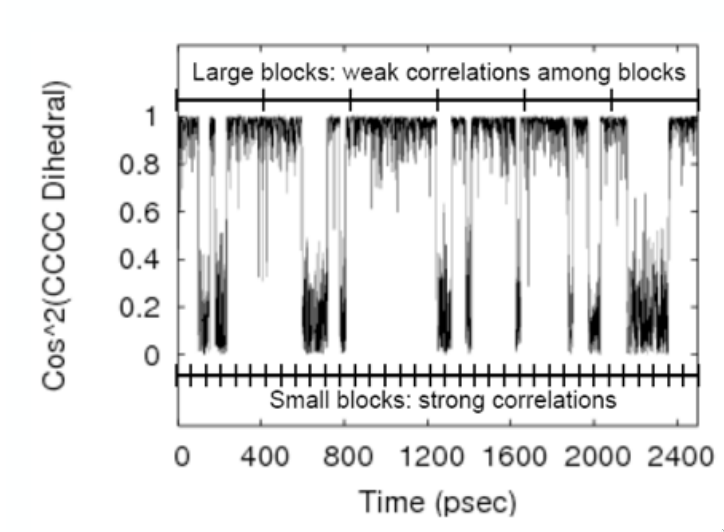
\includegraphics[width = 0.45\textwidth]{block-length}
		\caption{Varying block length}
		\label{fig:block-length}
	\end{figure}

	\columnbreak

	\begin{figure}[H]
		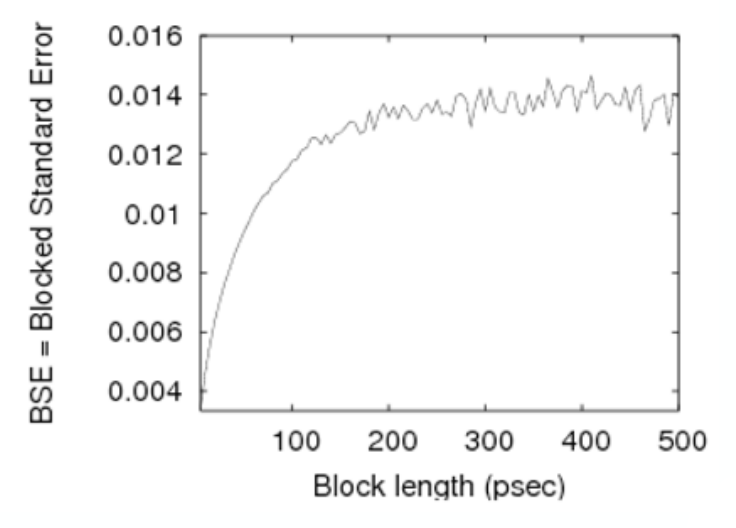
\includegraphics[width = 0.45\textwidth]{bse}
		\caption{BSE at varying block length}
		\label{fig:bse}
	\end{figure}

\end{multicols}
